\section{Projektstrukturplan}

\subsection{5. Semester}

Für das fünfte Semester wurde ein \gls{psp} erstellt. Auf Grund dessen Größe ist dieser nicht in diesem Dokument, sondern im Anhang eingefügt. Dieser \gls{psp} beinhaltet die in \vref{organigramm_semester5} abgebildeten Arbeitsgruppen, deren einzelne Aufgaben während des kompletten fünften Semesters, der geschätzte und der tatsächliche Arbeitsaufwand für die einzelnen Aufgaben.

\subsection{6. Semester}

Das sechste Semester wurde gleichermaßen in einem \gls{psp} zusammengefasst, dieser ist ebenfalls im Anhang abgelegt. Enthalten in diesem \gls{psp} sind die in \vref{organigramm_semester6} abgebildeten Arbeitsgruppen und deren Pflichten gegenüber des Projektteams. Nicht enthalten in der Übersicht sind die einzelnen Arbeitspakete der vier Arbeitsgruppen (Single-Purpose-Webapp, Newsfeed App Research, Captive Portal und Dokumentation). Für die Single-Purpose-Webapp (Lunchapp) und das Captive Portal wurden jeweils spezifische Arbeitspakete definiert und ein eigener \gls{psp} erstellt. Diese sind als beigefügt Dateien in diesem Dokument abgebildet. Für die nicht-technischen Aufgaben war es aufgrund der jeweils kleinen Teamgröße und klaren Zielen nicht nötig eigene Arbeitspakete oder einen \gls{psp} zu definieren. 

\subsection{Kanbanboard}

Nach der Erstellung des \gls{psp} wurde daraus innerhalb der Webanwendung Trello ein Kanbanboard erstellt (siehe \ref{fig:frame:kanban}). In diesem Kanbanboard werden jedem Arbeitspaket die verantwortlichen Personen, die benötigten Dateien, der Bearbeitungszeitraum und auch der Bearbeitungsstatus zugeordnet werden. Hierdurch ist der Fortschritt des Projekts und die zu bearbeitenden Aufgaben für alle Mitglieder einsehbar. Durch die Möglichkeit, Kommentare zu einzelnen Arbeitspaketen hinzuzufügen, kann direktes Feedback für Aufgaben anderer Teammitglieder gegeben werden und die gebrauchte Arbeitszeit eingetragen werden. Die gezielte Nutzung dieser Möglichkeit vereinfachte das Projektmanagement erheblich.

\begin{figure}[H]
\centering
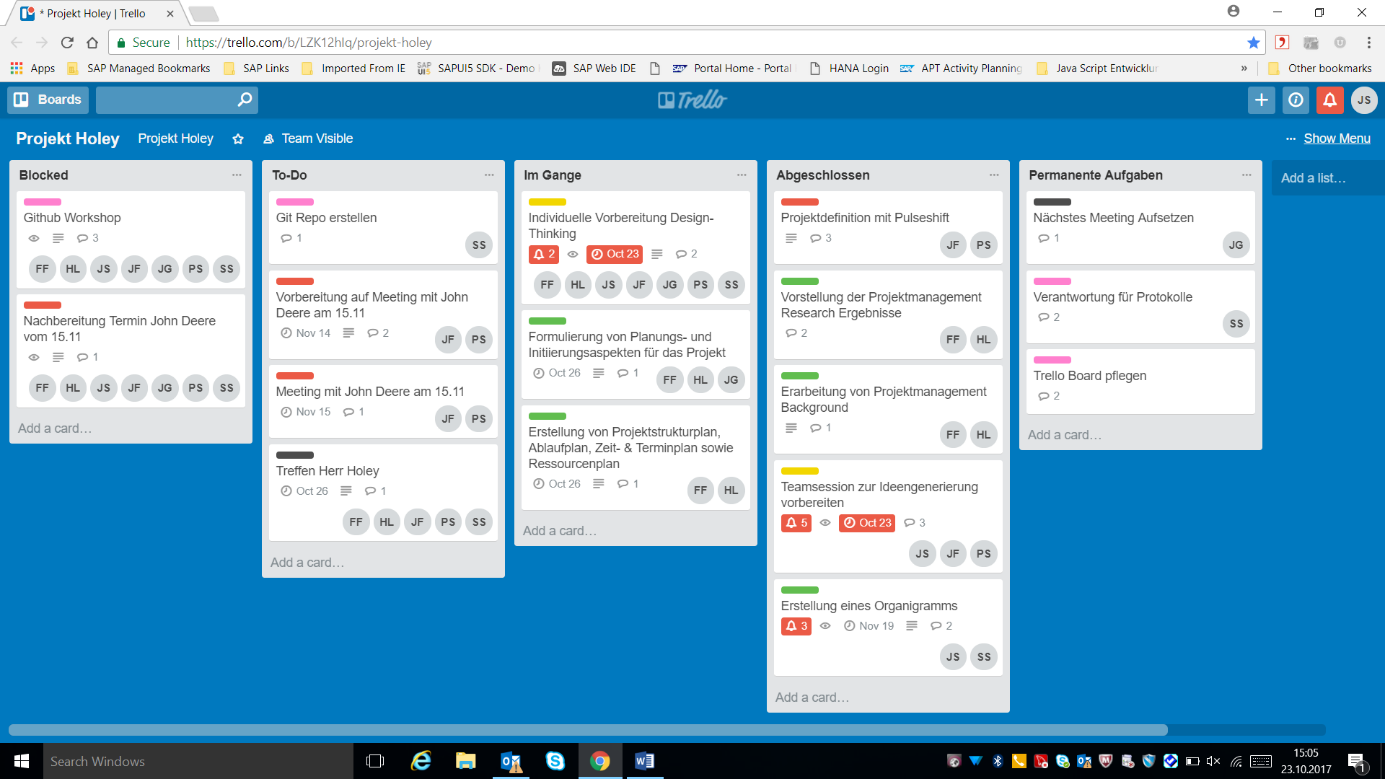
\includegraphics[width=1\textwidth]{images/trello}
\caption[Bildschirmabgriff des Kanbanboards in Trello]{Bildschirmabgriff des Kanbanboards in Trello}
\label{fig:frame:kanban}
\end{figure}
